%++++++++++++++++++++++++++++++++++++++++
% Don't modify this section unless you know what you're doing!
\documentclass[letterpaper,12pt]{article}
\usepackage[ngerman,english]{babel}
\usepackage{siunitx} 
\usepackage{tabularx} % extra features for tabular environment
\usepackage{amsmath}  % improve math presentation
\usepackage{graphicx} % takes care of graphic including machinery
\usepackage[margin=1in,letterpaper]{geometry} % decreases margins
\usepackage{cite} % takes care of citations
\usepackage[final]{hyperref} % adds hyper links inside the generated pdf file
\hypersetup{
	colorlinks=true,       % false: boxed links; true: colored links
	linkcolor=blue,        % color of internal links
	citecolor=blue,        % color of links to bibliography
	filecolor=magenta,     % color of file links
	urlcolor=blue         
}
%++++++++++++++++++++++++++++++++++++++++


\begin{document}
	
	\selectlanguage{ngerman}
	\title{Hochfrequenzchirurgie}
	\author{Heinrich Merk}
	\date{\today}
	\maketitle
	
	\selectlanguage{english}
	\begin{abstract}
		In dieser Ausarbeitung geht es um die Hochfrequenzchirurgie und derer grundlegenden physikalischen Prozesse. Es werden die verschiedenen Auswirkungen auf das Gewebe, die Apparatur sowie das grundlegende Verständis zur dahinter liegenden Technik beleuchtet. Zum Schluss werden neu erworbene Techniken aufgegriffen und Aussichtsmöglichkeiten vorgestellt.
		
	\end{abstract}
	
	\selectlanguage{ngerman}
	\section{Einleitung}
	
		Unter der Hochfrequenzchirurgie versteht man den assistierenden Einsatz von elektrischer Energie in der Chirurgie zur thermisch induzierten Veränderung oder Zerstörung von Gewebezellen mit dem Ziel der Hämostase (Blutstillung), Gewebedurchtrennung oder -versiegelung \cite{kramme2016medizintechnik}. Durch die kompakte Größe der Geräte, die einfache Handhabung und der Preiswertigkeit hat sich die HF-Chirurgie zu einem unentbehrlichen Handwerkszeug im operativen Alltagsbereich entwickelt und ist kaum noch wegzudenken.
	
	\section{Stand der Technik}
	
		Die HF-Chirurgie lässt sich grundsätzlich auf drei wichtige Bauteile, dem Hochfrequenzgenerator, dem Applikator und der Erdung beschränken. Hierbei sorgt der HF-Generator für den benötigten Wechselstrom in einer wohl definierten Frequenz. Diese sind in der Lage eine Frequenz von $f>\SI{300}{\kilo\hertz}$ zu betreiben. Applikatoren als Handwerkszeug und Stromspitze können je nach Anwendung in verschiedenen Bauformen auftreten. Hier kann ein isoliertes Handstück diverse Applikatorspitzen für den jeweiligen Einsatz aufnehmen. Die Erdung erfolgt mithilfe einer großflächigen Elektrode oder aber der Patientenstuhl ist als Erdung direkt konfiguriert. 
		
	
	\newpage
	\section{Grundlagen}
	
		\subsection{Thermische Prozesse im Gewebe}
		
		Das Gewebe besteht grundsätzlich aus Proteinbausteinen, welche durch Temperaturerhöhung eine veränderte Form erfahren. Dabei sind folgende Stufen für die Hochfrequenzchirurgie von Relevanz:
		\begin{itemize}
			\item $37^\circ-45^\circ$ $\Rightarrow$ Erwärmung des Gewebes
			\item $45^\circ-70^\circ$ $\Rightarrow$ Proteindenaturierung (3D-Struktur der Proteine geht verloren, d.h. auch ihre Funktion)
			\item $70^\circ-100^\circ$ $\Rightarrow$ Austrocknung/Koagulation (Verklumpen von Proteinen)
			\item $100^\circ-300^\circ$ $\Rightarrow$ Karbonisation (Gewebe färbt sich schwarz)
			\item über $300^\circ$ $\Rightarrow$ Verdampfen und Abtragung des Gewebes
		\end{itemize}
		Bereits bei der Proteindenaturisierung sterben die Zellen ab und sind nicht mehr in der Lage sich selbstständig zu regenerieren. Die anschließende Koagulation findet Einsatz in der Blutstillung. Durch das verklumpen der Proteine wird eine Blutgerinnung verhindert...
	
		\subsection{Elektrische Wechselwirkung mit dem Gewebe}
	
			Fließt ein elektrischer Strom durch biologisches Gewebe, treten je nach Stromart, Stromstärke und Frequenz drei unterschiedliche Effekte auf:
			\paragraph{Gleichstrom ($f=\SI{0}{\hertz}$)}
			Gleichstrom hat für das Gewebe eine elektrolytische Wirkung. Es folgt eine Ionenverschiebung und elektrochemische Prozesse treten in Kraft. 
			\paragraph{Wechselstrom ($f=\SI{20}{\hertz}-\SI{20}{\kilo\hertz}$)}
			Bei diesen Frequenzen treten faradische Effekte auf. Diese sorgen für eine Störung der Nerven- und Muskelreizung. Gefährlich sind solche Frequenzen insbesondere für das Herz, da diese es kontrahieren lassen und Herzrythmusstörungen zur Folge haben.
			\paragraph{Wechselstrom ($f>\SI{300}{\kilo\hertz}$)}
			Derartige Frequenzen lassen thermische Effekte zu. Die elektrische Energie kann effektiv übertragen werden, da hohe Frequenzen für eine hohe Leitfähigkeit im Gewebe sorgen, das vor allem einen kapazitiven Widerstand hat.\\\\	
			Die Erwärmung des Gewebes ist abhängig von der Stromdichte, welche wie folgt definiert ist:
			\begin{equation} \label{eq:stromdichte}
				S=\frac{I}{A}
			\end{equation}
			Die Einwirkfläche $A$ wird von der Geometrie der Applikatoren, welche letztendlich mit der Haut in Kontakt kommen, bestimmt. Eine spitze Form sorgt für eine kleine Fläche und folglich einer hohen Stromdichte $S$. Anwendungsgebiet ist das Schneiden von Gewebe. Eine beispielsweise kugelförmige Geometrie sorgt hingegen für eine geringere Stromdichte. Dadurch kann eine Koagulation des Gewebes erfolgen.\\Der Strom $I$ hängt ab vom spezifischen Widerstand des Gewebes und der verwendeten Effektivspannung
			\begin{equation} \label{eq:effektivspannung}
			U_{effektiv}=R_{Gewebe}*I.
			\end{equation}
			Auch die Einwirkzeit hat einen Einfluss auf die Erwärmung des Gewebes. Je länger der Wärmefluss ins Gewebe andauert, desto höher ist der Temperaturanstieg. Mit steigender Temperatur ändert sich wiederum der Gewebezustand.
		
		
	\section{Anwendung}
	
		\subsection{Bipolare Technik}
		
		\subsection{Monopolare Technik}
	
	
	\section{Vor- und Nachteile}
	
	In this section you will need to show your experimental results. Use tables and
	graphs when it is possible. Table~\ref{tbl:bins} is an example.
	
	\begin{table}[ht]
		\begin{center}
			\caption{Every table needs a caption.}
			\label{tbl:bins} % spaces are big no-no withing labels
			\begin{tabular}{|cc|} 
				\hline
				\multicolumn{1}{|c}{$x$ (m)} & \multicolumn{1}{c|}{$V$ (V)} \\
				\hline
				0.0044151 &   0.0030871 \\
				0.0021633 &   0.0021343 \\
				0.0003600 &   0.0018642 \\
				0.0023831 &   0.0013287 \\
				\hline
			\end{tabular}
		\end{center}
	\end{table}
	
	Analysis of equation~\ref{eq:aperp} shows ...
	
	Note: this section can be integrated with the previous one as long as you
	address the issue. Here explain how you determine uncertainties for different
	measured values. Suppose that in the experiment you make a series of
	measurements of a resistance of the wire $R$ for different applied voltages
	$V$, then you calculate the temperature from the resistance using a known
	equation and make a plot  temperature vs. voltage squared. Again suppose that
	this dependence is expected to be linear~\cite{Cyr}, and the proportionality coefficient
	is extracted from the graph. Then what you need to explain is that for the
	resistance and the voltage the uncertainties are instrumental (since each
	measurements in done only once), and they are $\dots$. Then give an equation
	for calculating the uncertainty of the temperature from the resistance
	uncertainty. Finally explain how the uncertainty of the slop of the graph was
	found (computer fitting, graphical method, \emph{etc}.)
	
	If in the process of data analysis you found any noticeable systematic
	error(s), you have to explain them in this section of the report.
	
	It is also recommended to plot the data graphically to efficiently illustrate
	any points of discussion. For example, it is easy to conclude that the
	experiment and theory match each other rather well if you look at
	Fig.~\ref{fig:samplesetup} and Fig.~\ref{fig:exp_plots}.
	
	\begin{figure}[ht] 
		\centering
		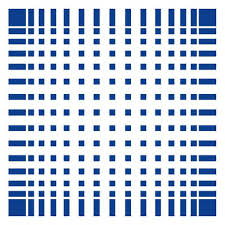
\includegraphics[width=0.5\columnwidth]{Images/hsMannheim.jpg}
		
		% some figures do not need to be too wide
		\caption{
			\label{fig:exp_plots}  
			Every plot must have axes labeled.
		}
	\end{figure}
	
	
	\section{Ausblick}
	In Zukunft wird sich zeigen, ob...
	



	\bibliographystyle{unsrt}
	\bibliography{Literatur}
	
	
\end{document}